\documentclass[a4paper]{article}
\usepackage[T1]{fontenc}
\usepackage[francais]{babel}
\usepackage{entete}
\usepackage{noitemsep}
\usepackage{euscript} 
\usepackage{amsmath,amssymb,amsfonts,amsthm}
\usepackage{graphicx,graphics,epsfig,subfigure,color}
\usepackage{url}
%\usepackage{algorithm2e}
\usepackage{multicol}
\usepackage{a4wide}
\usepackage{latexsym}
\usepackage{verbatim}
\setlength{\textheight}{23.6cm}
\setlength{\topmargin}{-1cm}
\setlength{\textwidth}{165mm}
\setlength{\oddsidemargin}{1.5mm}
\usepackage[utf8]{inputenc}
\usepackage{eurosym}

\usepackage{pdfpages}
%\renewcommand{\baselinestretch}{0.85}

\pagenumbering{gobble}  %% remove page number

%\input{macroAlgo}
%\dontprintsemicolon

\setlength{\parindent}{0pt}  %%suppression indentation

\newif\ifcorrection
\correctiontrue   %% With correction
\correctionfalse   %% Reviewer's version


\begin{document}
\selectlanguage{francais}
\author{D. Fourer, L. Lagon}
\newcommand{\universityname}{IUT d'\'Evry Val d'Essonne}
\newcommand{\deptname}{D\'epartement TC (S3)}
\newcommand{\years}{2023-2024}

%------------------- TITRE -----------------------------------------
\date{Septembre 2021} 
\TDHead{\universityname}{\deptname}{R1.07, \years}{\large DS2: Mathématiques}
%\TDHead{DUT TC}{}{\large TIC3: Fonctions avanc\'ees d'un tableur}
%-------------------------------------------------------------------
\vspace{-0.5cm}

\begin{center}
 \textbf{Dur\'ee 1h30, documents et objets connect\'es interdits. Calculatrice autorisée. }\\
 \textit{Chaque r\'eponse devra \^etre r\'edig\'ee en fran\c{c}ais, \^etre intelligible et parfaitement justifi\'ee.}\\% (1 point de pr\'esentation)}
\end{center}


\exost Questions de cours ( points): 


\vspace{0.4cm}
\exost Taux d'évolution
\begin{enumerate}
    \item Entre 2022 et 2023, le prix de l’abonnement Navigo est passé de 75,20 \euro\ à 84,10 \euro. Calculer son taux d’évolution.

\vspace{0.2cm}

    \item Entre Septembre 2023 et Décembre 2023, le prix moyen du litre d’essence est passé de 1,99\euro\ à 1,78\euro. Calculer son taux d’évolution.

\vspace{0.2cm}

    \item Sur les 6 derniers mois, la valeur d’une action de l’entreprise Tesla a perdu 7,63\%. Son prix initial était de 253,50\$. Quelle est la valeur actuelle de cette action ?

\vspace{0.2cm}

    \item En mars 2021, un paquet de spaghettis coûtait 0,77€. Il a subi depuis une augmentation de 42\%. Quelle est la valeur de son prix aujourd’hui ?

\end{enumerate}


\vspace{0.4cm}
 \exost Taux d'évolution global

 Au cours de l’année, l’action LVMH, dont le prix initial était de 700\euro\, a augmenté de 29\%, puis a diminué de 26\%, puis a ré-augmenté de 12\%.

\begin{enumerate}
    \item Calculer le prix final de l'action.

\vspace{0.2cm}

    \item Calculer le taux d'évolution global de l'action. 

\vspace{0.2cm}
\end{enumerate}


\vspace{0.4cm}
\exost Taux d'évolution moyen

Le graphique ci-dessous donne l’évolution du prix annuel d’un paquet de cigarettes entre 2000 et 2021.

\begin{figure}[h] 
  \centering
  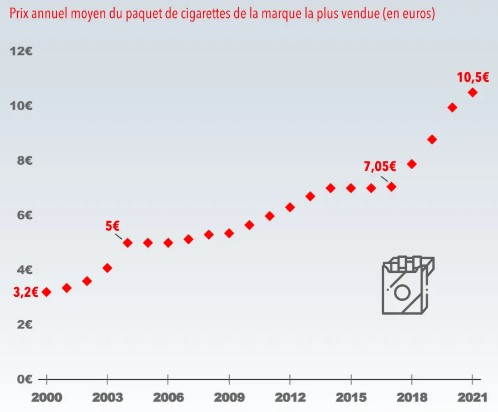
\includegraphics[width=0.5\textwidth]{cigarettes.jpg} 
\end{figure}


\begin{enumerate}
    \item Déterminer le taux d'évolution global entre les années 2000 et 2021.
    \item Déterminer le taux d'évolution moyen entre les années 2000 et 2021.
    \item En supposant ce taux constant sur les 20 prochaines années, calculer le prix d'un paquet de 2041. 

\vspace{0.2cm}
\end{enumerate}


\vspace{0.5cm}
\exost Suite à intérêts composés 

Un étudiant dépose la somme de 1000 \euro\ sur un livret A. Ce livret rapporte 3\% chaque année. On suppose que le taux reste stable et que les intérets sont réintégrés au capital.

De quelle somme d'argent disposera cet étudiant dans 10 ans ?

\end{document}

% End Of File

